\chapter{Desarrollo}
\label{chap:desarrollo}

\drop{C}{  omo} ya se ha comentado antes, el desarrollo de este proyecto ha supuesto un reto importante ya que las tecnologías utilizadas eran totalmente desconocidas. En este capítulo se explica el proceso seguido a lo largo de su desarrollo, además de presentar los principales problemas encontrados y las soluciones con las que se han abordado.

\section{Entrega 0}

El objetivo de esta primera entrega fue, por un lado, establecer la estructura principal del proyecto y esbozar una primera versión del a narrativa y por otro realizar una primera toma de contacto con el desarrollo de Unity, las tecnologías \acs{VR} e instalar y configurar el entorno de desarrollo para poder empezar a trabajar en la siguiente entrega.

\subsection{Estructuración del proyecto}

El primer paso lógico tras proponerle a mi tutor el proyecto y ser éste aprobado fue empezar a definirlo. Para ello, y partiendo de la idea principal de desarrollar una experiencia de juego haciendo uso de tecnologías \acs{VR} que pusiera en contacto con el mundo del arte a personas que suelen y no visitar museos, generé el documento que puede verse en el anexo \ref{anexo:guia-salas}. 

Este documento comienza a detallar la narrativa del juego y la integra en una visita por un museo ficticio y, aunque terminó por sufrir varios cambios importantes, sirvió para definir el punto de partida del proyecto.

A lo largo de este documento se intenta crear una historia interesante para el jugador al mismo tiempo que generar un museo ficticio pero realista y coherente en el que se pueda desarrollar dicha narrativa. Para ello, se ha seguido el orden cronológico por las épocas más importantes en la historial de arte, definiendo una sala con una historia diferente para cada una.

A la hora de elegir los cuadros que se mostrarían en las salas se intentó buscar aquellos más representativos de su época. Para ello, se contó con el asesoramiento de una historiadora del arte, que ha sido quien ha dado el visto bueno al rigor artístico del museo.

\subsection{Configuración del entorno de desarrollo}

Antes de poder empezar a desarrollar el proyecto fue necesario elegir un \acs{IDE} y un framework con el que trabajar. Como ya se ha explicado en los capítulos \ref{chap:estado_arte} y \ref{chap:tecnologia}, tras comparar las ventajas y desventajas de los entornos de desarrollo y librerías disponibles en el mercado se decidió trabajar con Unity, el framework \acs{VRTK} y la librería SteamVR, para lo que hubo que importarlas manualmente al proyecto de Unity.

\section{Entrega 1}

Como se indicó en el capítulo \ref{chap:plan_entregas}, el objetivo final de las iteraciones de esta entrega fue aprender a importar modelos a Unity desde Blender y diseñar e implementar el tutorial del proyecto y que éste fuera completamente funcional. 

\subsection{Modelado e importación}

Lo primero que se hizo antes de comenzar a modelar en Blender, ya que es mucho menos productivo empezar a trabajar sin una idea previa, fue diseñar un boceto en papel en el poder basar el modelado posterior.

Como se consideró que el museo sería más realista si en lugar de empezar directamente en él el jugador tuviera que recorrer un pequeño pasillo que funcionara de antesala y desde el que se pudiera ver el exterior, fue el primer boceto que se hizo, y tras él se dibujó la sala que actuaría de tutorial. Esta sala tendría que presentar un cuadro muy reconocible y una pequeña prueba relacionada con él, por lo que se decidió utilizar el cuadro \textit{El Hijo del Hombre} de René Magritte (1964) y que el jugador tuviera que cambiar de sitio una pieza de fruta relacionada con este cuadro, de este modo aprendiendo que puede interaccionar con los elementos virtuales y que habrá relación entre las pruebas y las obras de arte de tal manera que el reto sea darse cuenta de estas ideas y no la prueba en sí. La imagen \ref{fig:bocetos-salas-0-1} muestra el boceto de estas dos salas, que fue dibujado antes de comenzar a modelarlas.

\begin{figure}[!h]
\begin{center}
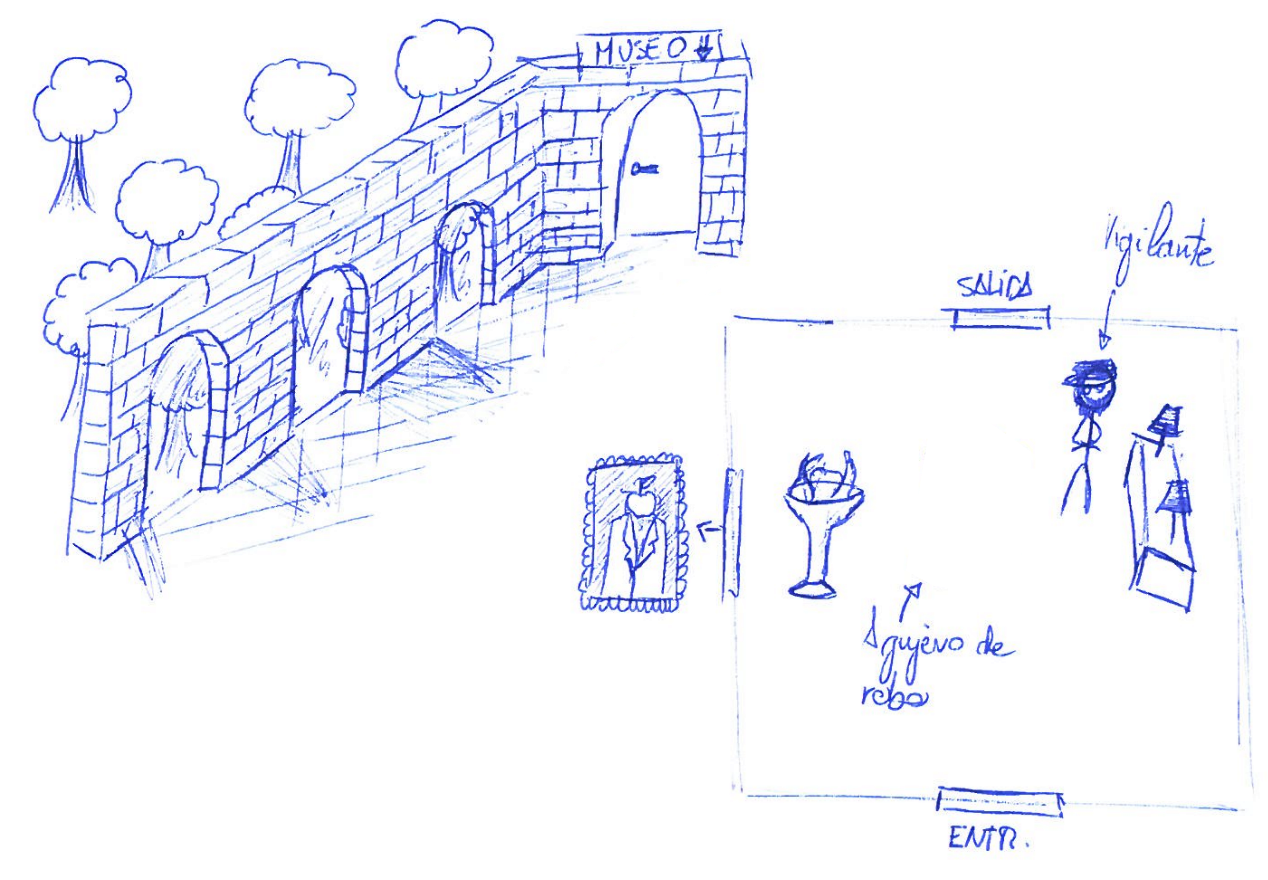
\includegraphics[width=1\textwidth]{imagenes/7/bocetos/boceto-sala-0-1.png}
\caption{Boceto de la antesala y la sala de tutorial}
\label{fig:bocetos-salas-0-1}
\end{center}
\end{figure}


\begin{figure}[!h]
\begin{center}
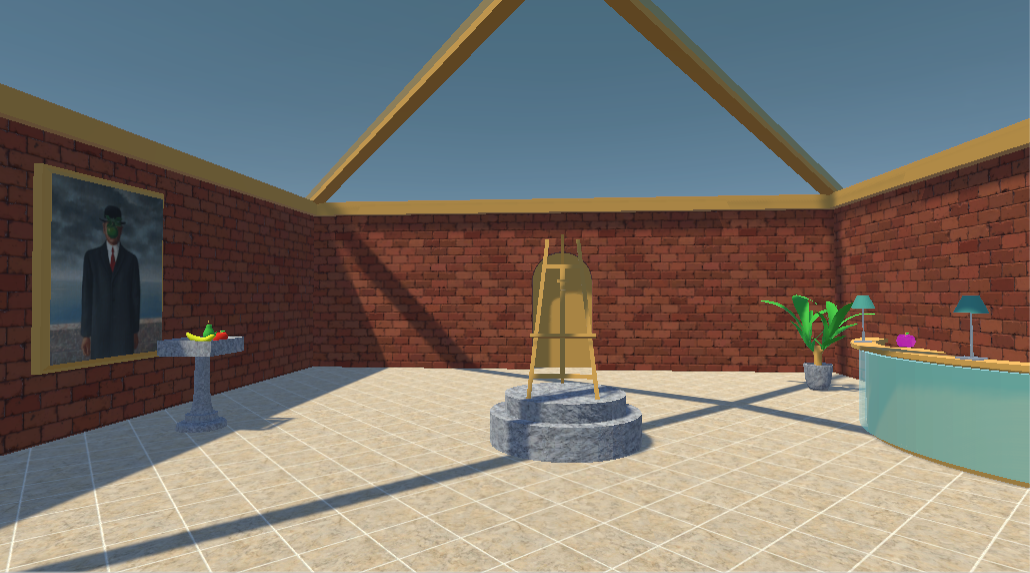
\includegraphics[width=1\textwidth]{imagenes/7/salas-unity/unity-sala-1.png}
\caption{Unity sala 1}
\label{fig:unity-sala-1}
\end{center}
\end{figure}

\subsection{Interacción con objetos virtuales}


\subsection{Viaje entre salas}


\section{Entrega 2}

\begin{figure}[!h]
\begin{center}
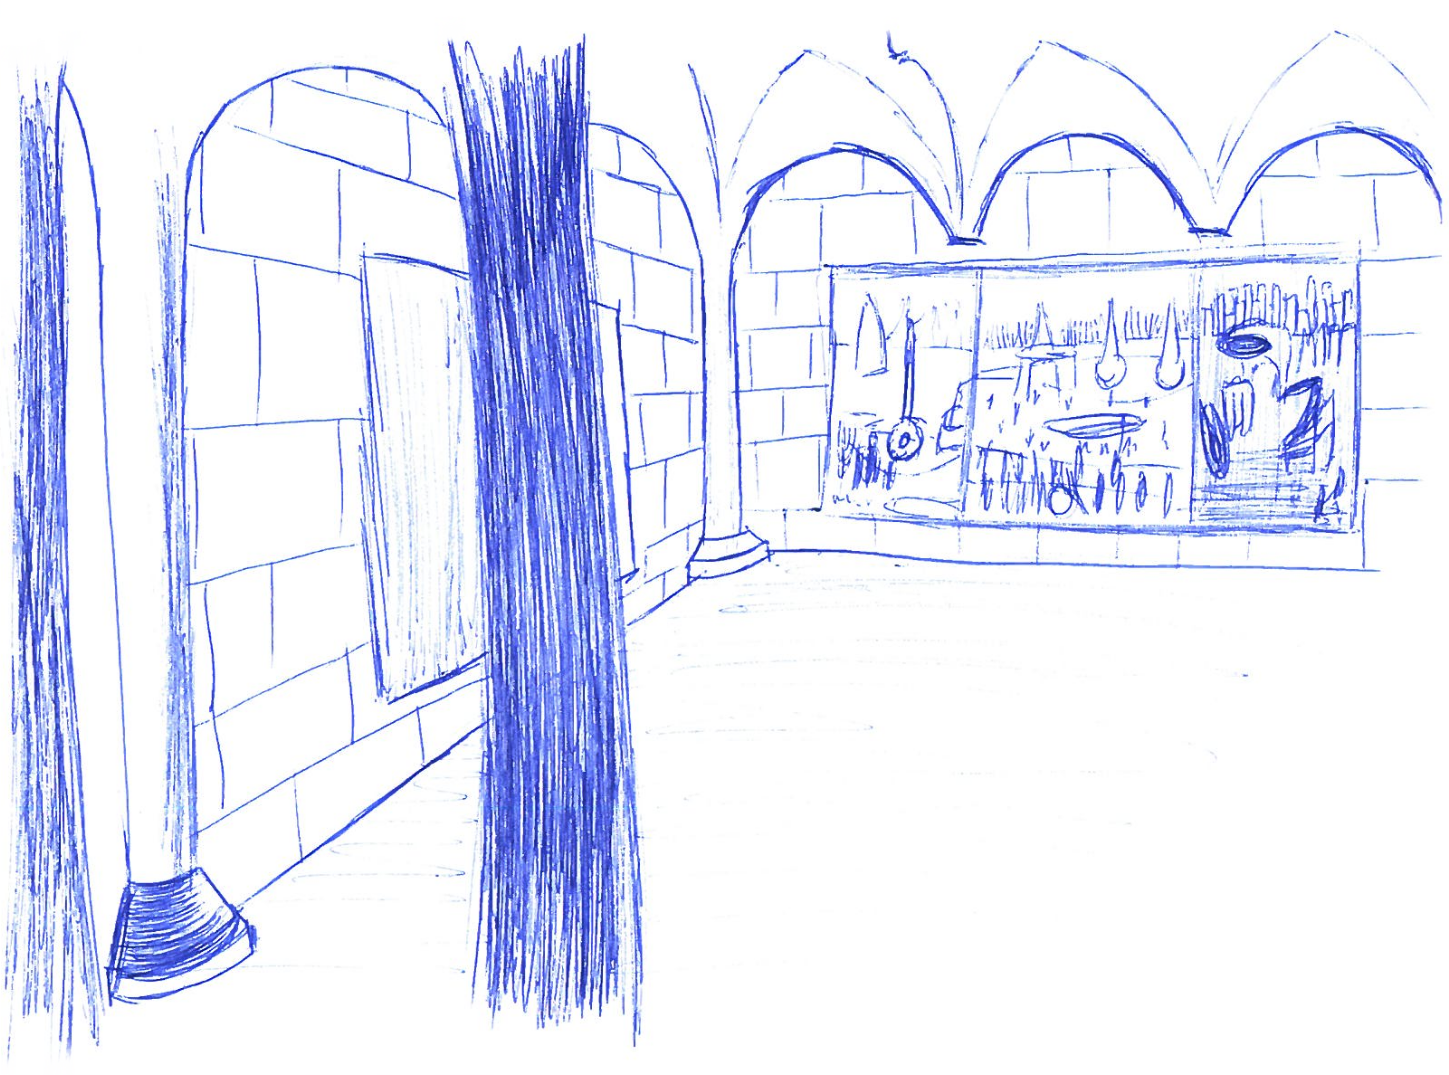
\includegraphics[width=1\textwidth]{imagenes/7/bocetos/boceto-sala-2.png}
\caption{Boceto de la segunda sala}
\label{fig:bocetos-salas-2}
\end{center}
\end{figure}

\section{Entrega 3}

\begin{figure}[!h]
\begin{center}
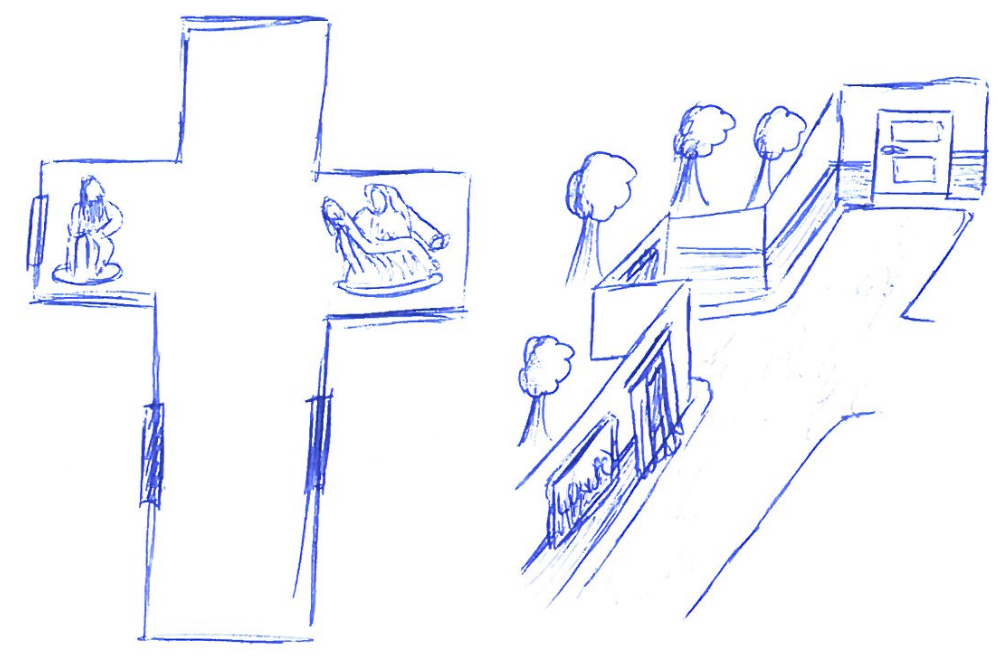
\includegraphics[width=1\textwidth]{imagenes/7/bocetos/boceto-sala-3.png}
\caption{Boceto de la tercera sala}
\label{fig:bocetos-salas-3}
\end{center}
\end{figure}

\section{Entrega 4}

\begin{figure}[!h]
\begin{center}
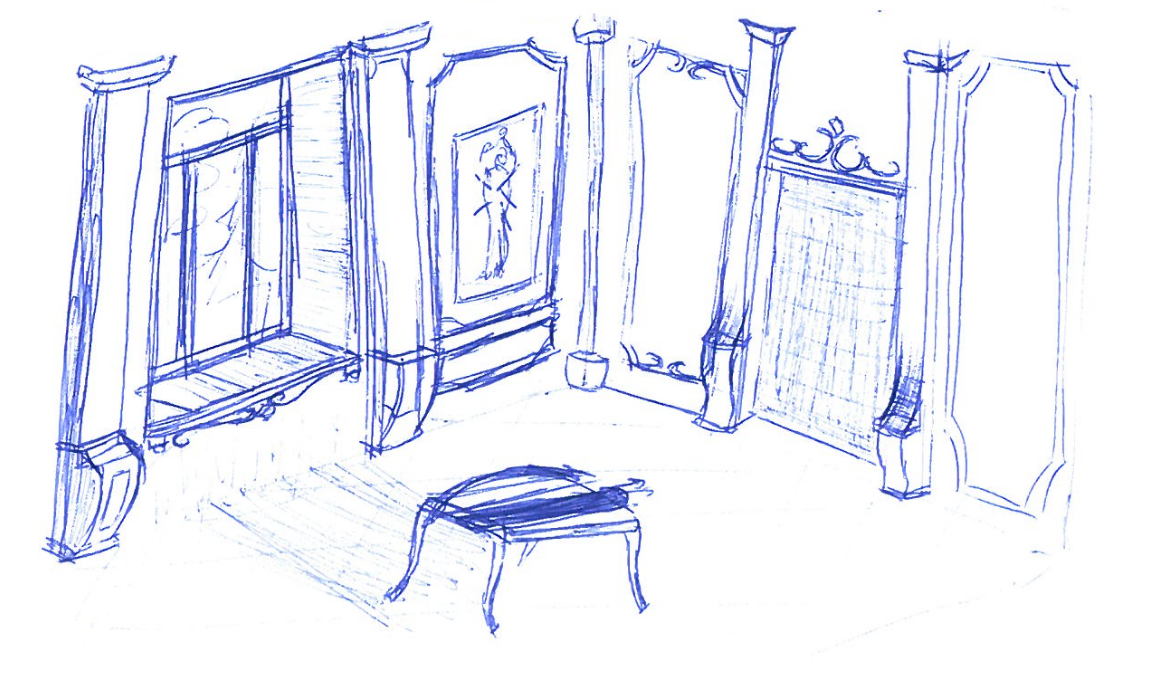
\includegraphics[width=1\textwidth]{imagenes/7/bocetos/boceto-sala-4.png}
\caption{Boceto de la cuarta sala}
\label{fig:bocetos-salas-4}
\end{center}
\end{figure}

\begin{figure}[!h]
\begin{center}
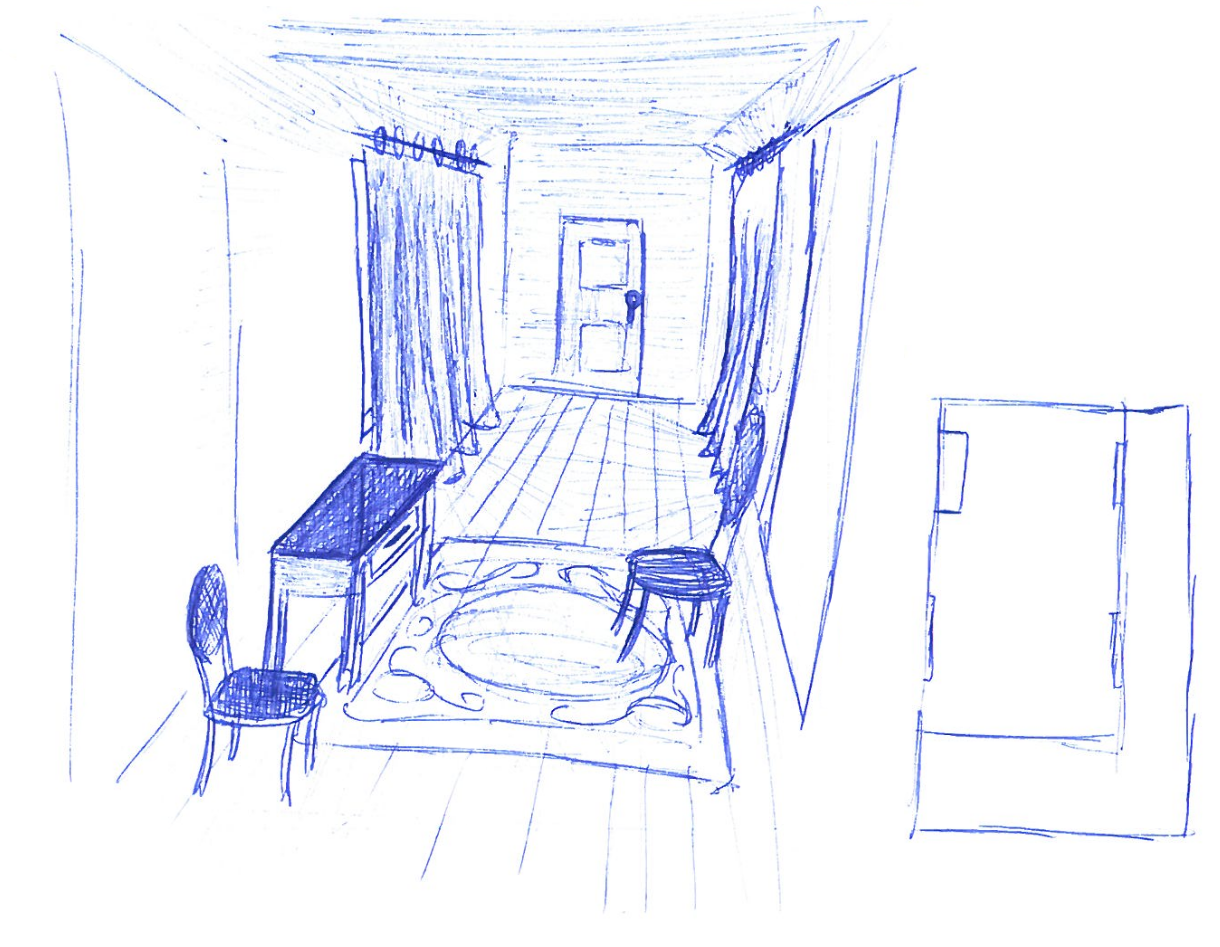
\includegraphics[width=1\textwidth]{imagenes/7/bocetos/boceto-sala-5.png}
\caption{Boceto de la quinta sala}
\label{fig:bocetos-salas-5}
\end{center}
\end{figure}

\section{Entrega 5}

\begin{figure}[!h]
\begin{center}
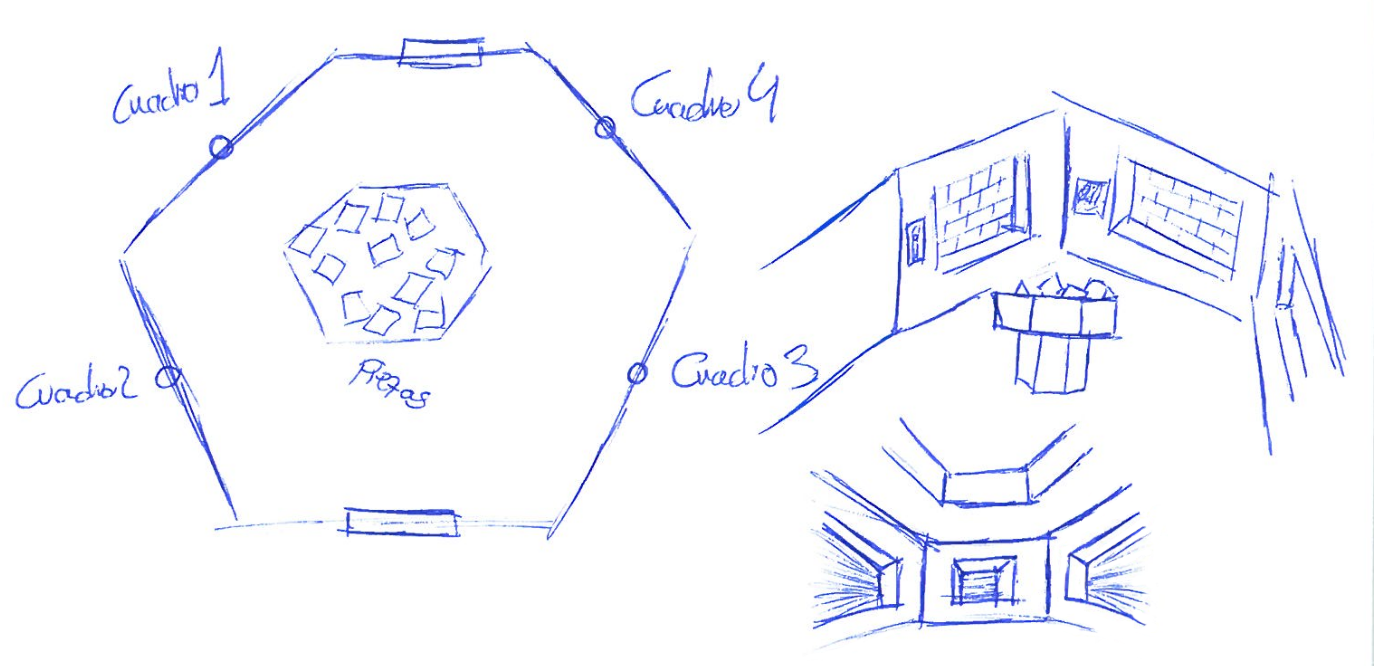
\includegraphics[width=1\textwidth]{imagenes/7/bocetos/boceto-sala-6.png}
\caption{Boceto de la sexta sala}
\label{fig:bocetos-salas-6}
\end{center}
\end{figure}

\section{Entrega 6}

